\chapter{Introduction}
\textit{ Why 802.15.4?}

\ac{sdr} are flexible radio platforms where most of the communication systems functionality is designed in software. Typically, \ac{sdr} platforms have on board radio front-end equipped with wide band antennas and analog signal processing chain for tuning the carrier frequency and desired bandwidth. High speed data converters convert the incoming analog signals into the digital domain and vice-versa. In traditional radios, the digital processing chain of a wireless protocol physical layer is implemented on the same chip as the radio front-end and analog signal processing functions. \ac{sdr}, on the other hand, in \textit{host-PHY(\cite{schmid_experimental_2007})} architecture transfers the converted data to a general purpose computing platform using bus transfer (USB, PCIe).  The digital processing chain is designed in software, thus allowing for flexibility in the protocol design, enabling experimentation in decoding and modulation techniques. \ac{sdr} also allows for careful analysis of RF signals as the raw sample data is made available to the host.\\

\begin{figure}[!h]
\centering
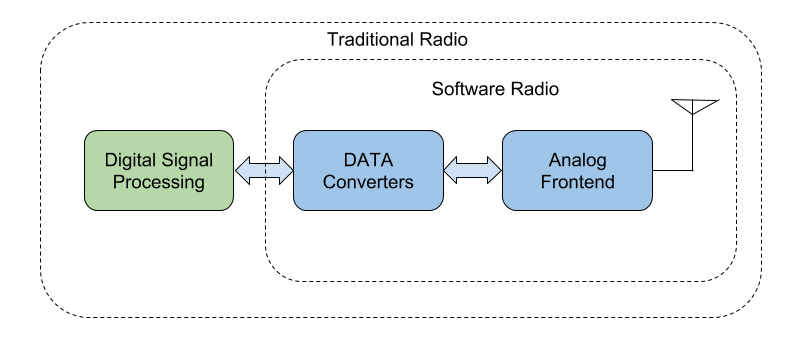
\includegraphics[width=0.75\textwidth]{Figure/SDRSystem.png}
\caption{Software Radio and Traditional Radio Architecture.}
\label{sdr_architecture}
\end{figure}


Communication systems needs to have longer service time in military sector as compared to commercial sector. \ac{sdr} helps to protect investments by facilitating change of protocols on already existing system. A major motivation within the commercial communications arena, is the rapid evolvement of communications standards, making software upgrades of base stations a more attractive solution than the costly replacement of base stations\cite{ulversoy_software_2010}. SDR also opens up the possibility of Cognitive Radios, a context sensitive radio system that can adapt depending on the radio channel conditions and applications. \\

A fundamental challenge of \ac{sdr} system is computational horsepower, because it needs to process complex data waveforms in a reasonable time-frame. Since \ac{sdr} involves transferring of signals and data from one system to another, this introduces considerable communication delays. Finally, general purpose processing systems introduces non-determinism in data processing and communication times.\\

Wireless devices share the wireless channel with other devices. Wireless protocol \ac{mac} layer is responsible for moderating access to the wireless channel. It typically uses \ac{tdma} and \ac{csma} to allocate the use of the channel. \ac{tdma} protocols schedule the allocation of the entire channel to one of the devices for a particular time duration. This requires global time synchronization among the devices so that the devices can understand when to transmit and receive. \ac{csma}, on the other hand uses the channel on an opportunistic basis, with the devices sensing if the channel is free or not. When it senses the channel to be free, it can start using it.  


\section{Problem Context}

\subsection{CSMA}
As highlighted by \cite{schmid_experimental_2007}, \ac{sdr} based systems don't comply the stringent timing constraints imposed by modern \ac{mac} protocols. Furthermore, the presence of long bus communication and latency delays creates \textit{blind spots}\cite{schmid_experimental_2007} in carrier sensing. In fig \ref{blind_spots}, a packet is being transmitted through the air medium which is received by the \ac{sdr} system. There is a delay being end of transmission ($t_0$) on the air medium and complete reception of packet ($t_1$) by the \ac{cpu} of the \ac{sdr} system. This delay is caused by processing and communication delay in a \ac{sdr} system. Once the packet has been received, the system wants to let the transmitting system about the successful reception using the \ac{ack} packet. Using carrier sensing it detects the medium is free, but this information is delayed by $t_1 - t_0$, hence the system is blind towards the real time channel situation when making the decision to transmit and might lead to a collision. \\ 

\begin{figure}[!h]
\centering
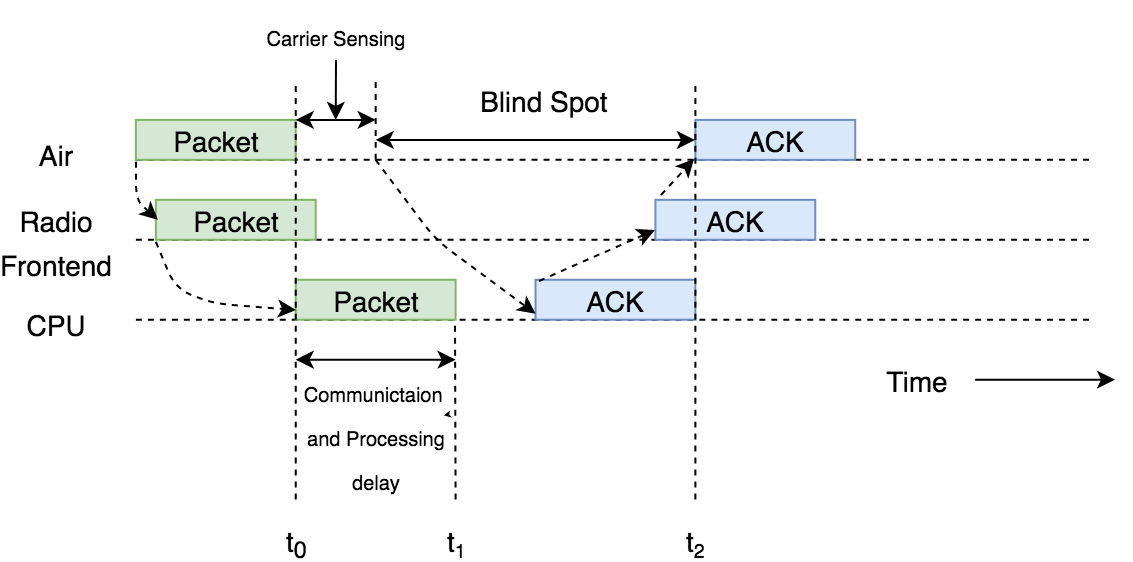
\includegraphics[width=0.6\textwidth]{Figure/BlindSpots.png}
\caption{Blind Spots Illustration(adapted from \cite{schmid_experimental_2007}).}
\label{blind_spots}
\end{figure}

Hence when designing \ac{mac} protocols, these delays needs to be taken into account, which necessitates a closer understanding of these delays and how different system parameters affect these delays.

\subsection{TDMA}
\ac{tdma} based protocols are controlled by time slots, hence there is need for precise scheduling to ensure that the transmissions happen in the correct time-slot. The delays and imprecise scheduling can be tolerated by making longer time-slots but that degrades the efficiency of the overall network. Modern contention based protocols(\ac{csma}) also require precise timing to implement inter-frame spacing.\\

Hence methods to implement precise time scheduling needs to studied.

\section{Research Questions}
\begin{itemize}
\item{ Quantitative evaluation of timing delays in \ac{sdr} systems.}
\begin{figure}[!h]
\centering
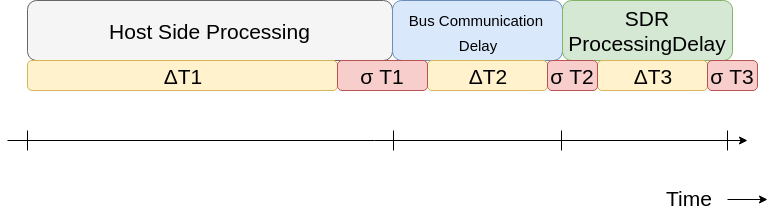
\includegraphics[width=0.75\textwidth]{Figure/RQ1.png}
\caption{Quantitative evaluation of timing delays.}
\label{rq1}
\end{figure}
\item{ Methods to implement precise scheduling in \ac{sdr} systems.}
\end{itemize}

\subsection{Report Outline}
The remainder of the report is structures as follows.\textit{Chapter 2} introduces the previous work in this field, as well the needed background information on the \ac{sdr} platform, the base system design and the relevant tools used in methods section. \textit{Chapter 3} introduces the experimental setup and the methods used in the measurement of the timing delays. \textit{Chapter 4} presents the experimental results, which are analyzed in \textit{Chapter 5}. Finally, \textit{Chapter 6} includes the concluding remarks and scope of future work.
